\documentclass[a4paper]{scrartcl}
\usepackage[utf8]{inputenc}
\usepackage[english]{babel}
\usepackage{graphicx}
\usepackage{lastpage}
\usepackage{pgf}
\usepackage{wrapfig}
\usepackage{fancyvrb}
\usepackage{fancyhdr}
\pagestyle{fancy}

% Create header and footer
\usepackage[backend=bibtex, citestyle=numeric-comp, bibstyle=ieee]{biblatex}
\addbibresource{ref.bib} % The file containing our references, in BibTeX format
\usepackage{hyperref}
\usepackage{listings}
\usepackage{subcaption}
\usepackage{enumitem}
\usepackage[section]{placeins}

% Create header and footer
\headheight 27pt
\pagestyle{fancyplain}
\lhead{\footnotesize{Internet Applications, ID1354}}
\chead{\footnotesize{Tasty Recipes with JavaScript}}
\rhead{}
\lfoot{}
\cfoot{\thepage\ (\pageref{LastPage})}
\rfoot{}

% Create title page
\title{Tasty Recipes with JavaScript}
\subtitle{Internet Applications, ID1354}
\author{Julius Recep Colliander Celik - jcelik@kth.se}
\date{\today}

\begin{document}

\maketitle

\section{Introduction}

This assignment was a continuation of the last one, where front-end interactivity was added to create a more fluent experience. Specifically JavaScript was used to introduce asynchronous interactions, where the window did not have to refresh for actions to be visible. The JavaScript framework React was used. To view the website it is publicly available on the link \href{https://github.com/juliuscc/kth-id1354/tree/master/homework-4}{https://github.com/juliuscc/kth-id1354/tree/master/homework-4}.

\section{Literature Study}

The React documentation was used for reference \href{https://reactjs.org/docs/}{https://reactjs.org/docs/}.

\section{Method}

I reused the code from the first assignment and modified it to achieve the tasks in this lab. I used VS Code as my text editor and used MAMP as a PHP web server and Database. I also introduced a Create React App project for development which later was extracted into another project that could enable the code to be used separately as a module on the page. Insomnia was used when developing the back-end API.

\section{Result}

I used the front-end framework React to implement a viewmodel sub-application, as I am familiar with React. To easily use one React app, instead of multiple apps that communicated with each other, I moved the login and register functionality to the comment section. Figure \ref{fig:comment-section} shows how the React app looks in different states.

\begin{figure}
	\centering
	\begin{subfigure}[b]{0.3\linewidth}
			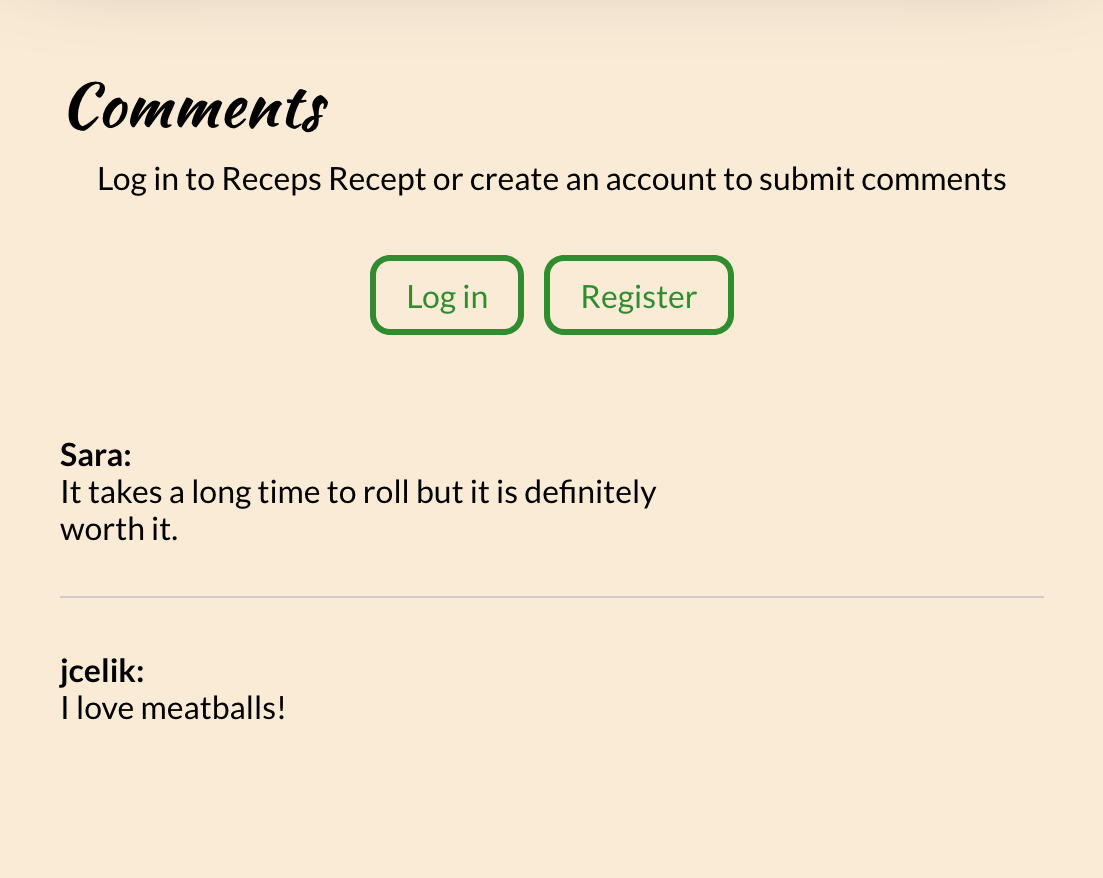
\includegraphics[width=\linewidth]{images/screenshot-comments-logged_out.png}
			\caption{Comment section with no user logged in.}
	\end{subfigure}
	\begin{subfigure}[b]{0.3\linewidth}
		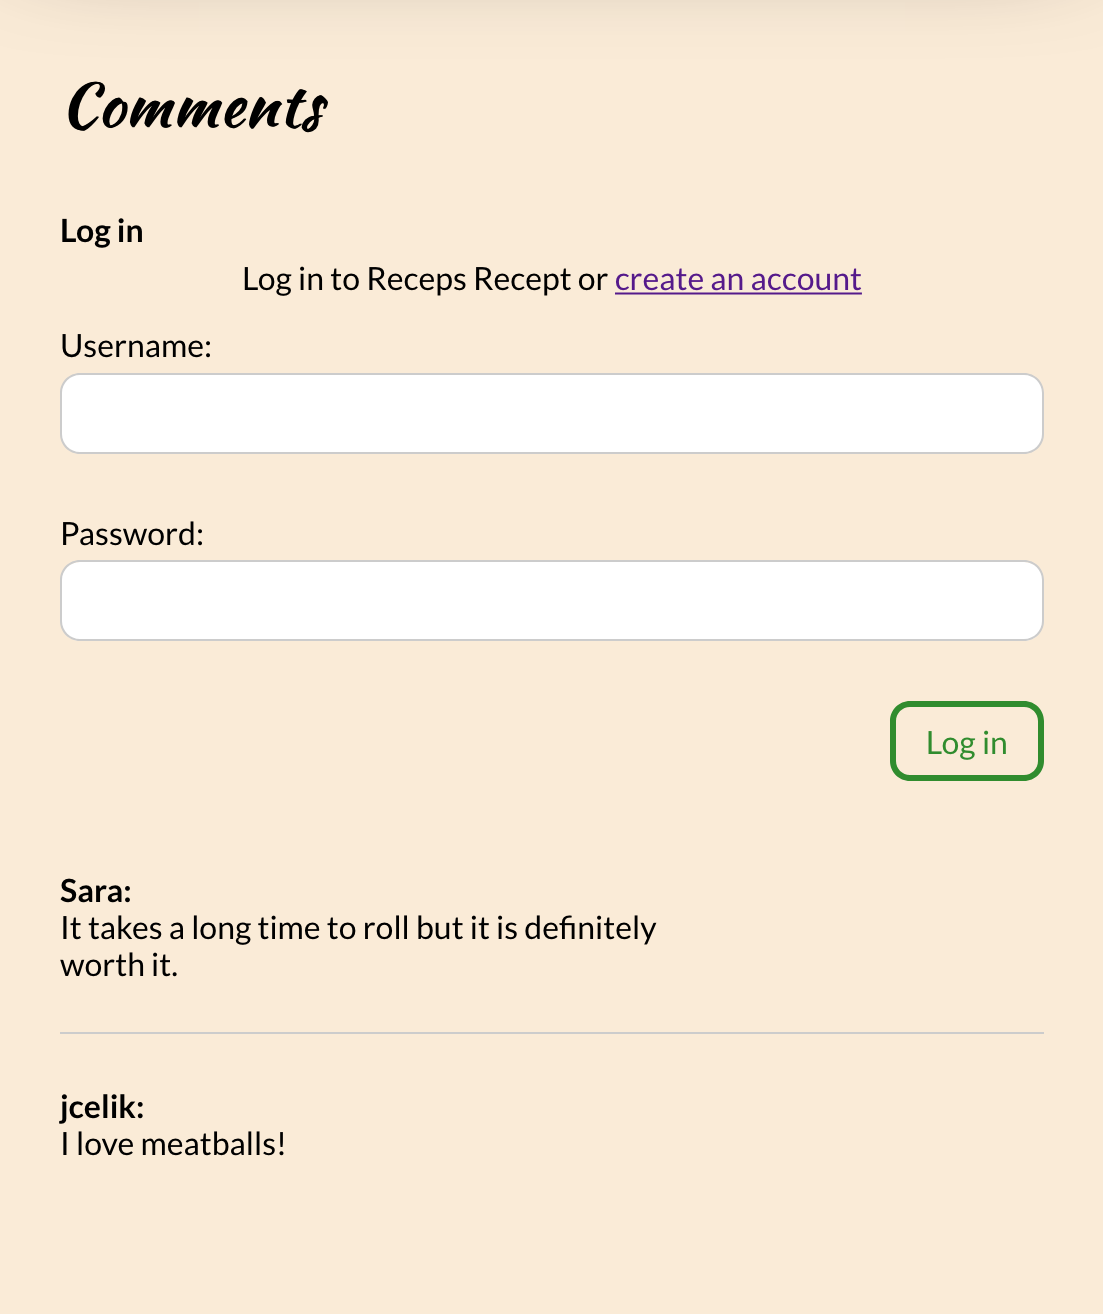
\includegraphics[width=\linewidth]{images/screenshot-comments-login.png}
		\caption{Comment section when logging in.}
	\end{subfigure}
	\begin{subfigure}[b]{0.3\linewidth}
		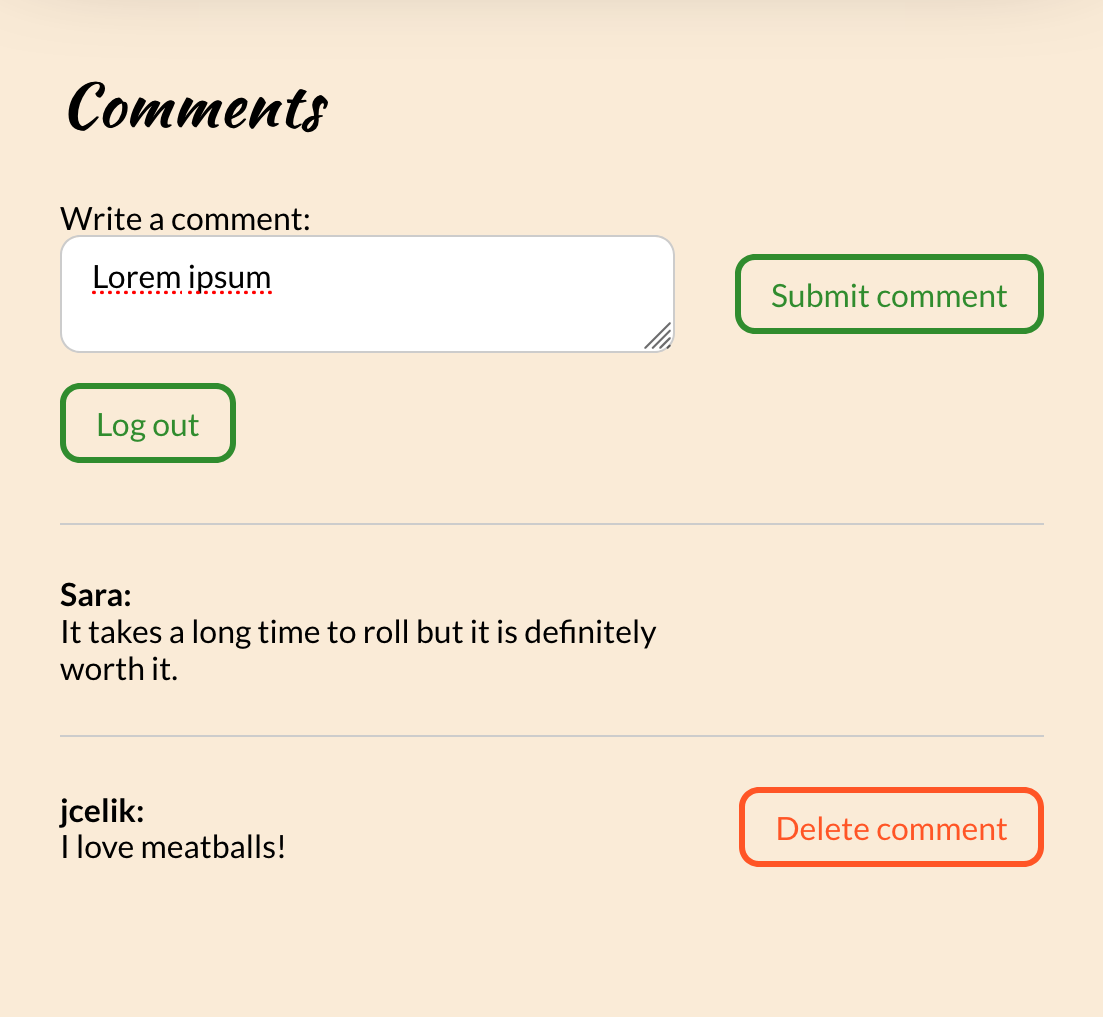
\includegraphics[width=\linewidth]{images/screenshot-comments-logged_in.png}
		\caption{Comment section when user is logged in.}
	\end{subfigure}
	\caption{Comment section with authentication implemented with React.}
	\label{fig:comment-section}
\end{figure}

\subsection{The viewmodel}
The viewmodel is implemented with React. React components hold a state, and depending on the state a view is rendered. It uses the observer pattern where any changes to the state triggers a re-render of the view. Figure \ref{fig:react-container} shows a wrapper container object that handles state and how it handles state. When the component is mounted, which happens once in the beginning of it's lifetime, the component fetches the state from the server which triggers the view to be re-rendered.

Figure \ref{fig:react-component} shows a comment component and how it is rendered from the properties it is given. Notice that this component can be a function as it is stateless while the wrapper container object is a class as it has to keep state.

\begin{figure}
	\begin{lstlisting}[frame=single, numbers=left, breaklines=true, basicstyle=\ttfamily\footnotesize, firstnumber=1]
import React, { Component } from 'react'
import './App.css'
import Wrapper from './components/CommentForm/CommentFormWrapper'
import CommentList from './components/Comments/Comment'

class App extends Component {
  constructor(props) {
    super(props)

    this.state = {}
  }

  componentDidMount() {
    fetch(this.props.apiUrl + '/comments/' + this.props.recipeId)
      .then(response => response.json())
      .then(json => this.setState({ comments: json }))

    const loggedInUser = localStorage.getItem('loggedInUser')
    this.setState({ loggedInUser })
  }
  .
  .
  .
	\end{lstlisting}
	\caption{Part of React component  (\href{https://github.com/juliuscc/kth-id1354/blob/master/homework-4/front-end/tasty_temp/src/App.js}{App.js}) that handles primary state}
	\label{fig:react-container}
\end{figure}

\begin{figure}
\begin{lstlisting}[frame=single, numbers=left, breaklines=true, basicstyle=\ttfamily\footnotesize, firstnumber=13]
const Comment = ({
  comment: { comment, id: comment_id, username, user_id },
  loggedInUser,
  deleteComment
}) => {
  return (
    <div className="user-comment">
      <div className="user-comment__wrapper">
        <div className="user-comment__username">{username}</div>
        <div className="user-comment__comment">{comment}</div>
      </div>
      <button
        type="submit"
        style={loggedInUser == user_id ? {} : { visibility: 'hidden' }}
        className="button button--danger"
        onClick={() => deleteComment(loggedInUser, comment_id)}
      >
        Delete comment
      </button>
    </div>
  )
}
\end{lstlisting}
	\caption{React component (\href{https://github.com/juliuscc/kth-id1354/blob/f811132bd5cd1c4ac30e0b60e7a2f64143a6d152/homework-4/front-end/tasty-app/components/Comments/Comment.js\#L13}{Comment.js}) for rendering a single comment.}
	\label{fig:react-component}
\end{figure}

\subsection{Fetch for authentication and storing authentication tokens}
When authenticating a user, a JSON object is sent and another JSON object is received. The JSON object sent contains the username and the password of the user, and the returning object contains the username and the user id. The user id is used as a login token however in a real application the token would be encrypted. Figure \ref{fig:api-login} shows a successful API call done with Insomnia.

The authentication token is both saved to the current state as well as saved in LocalStorage. When the application starts, the wrapper container object queries local storage for the authentication token, which in turn is saved in state. This can be seen on row 18 and 19 in figure \ref{fig:react-container}. Using LocalStorage ensures that the user is persistently authenticated even after refreshing a window, or visiting another page on the web site.

\begin{figure}
	\begin{center}
		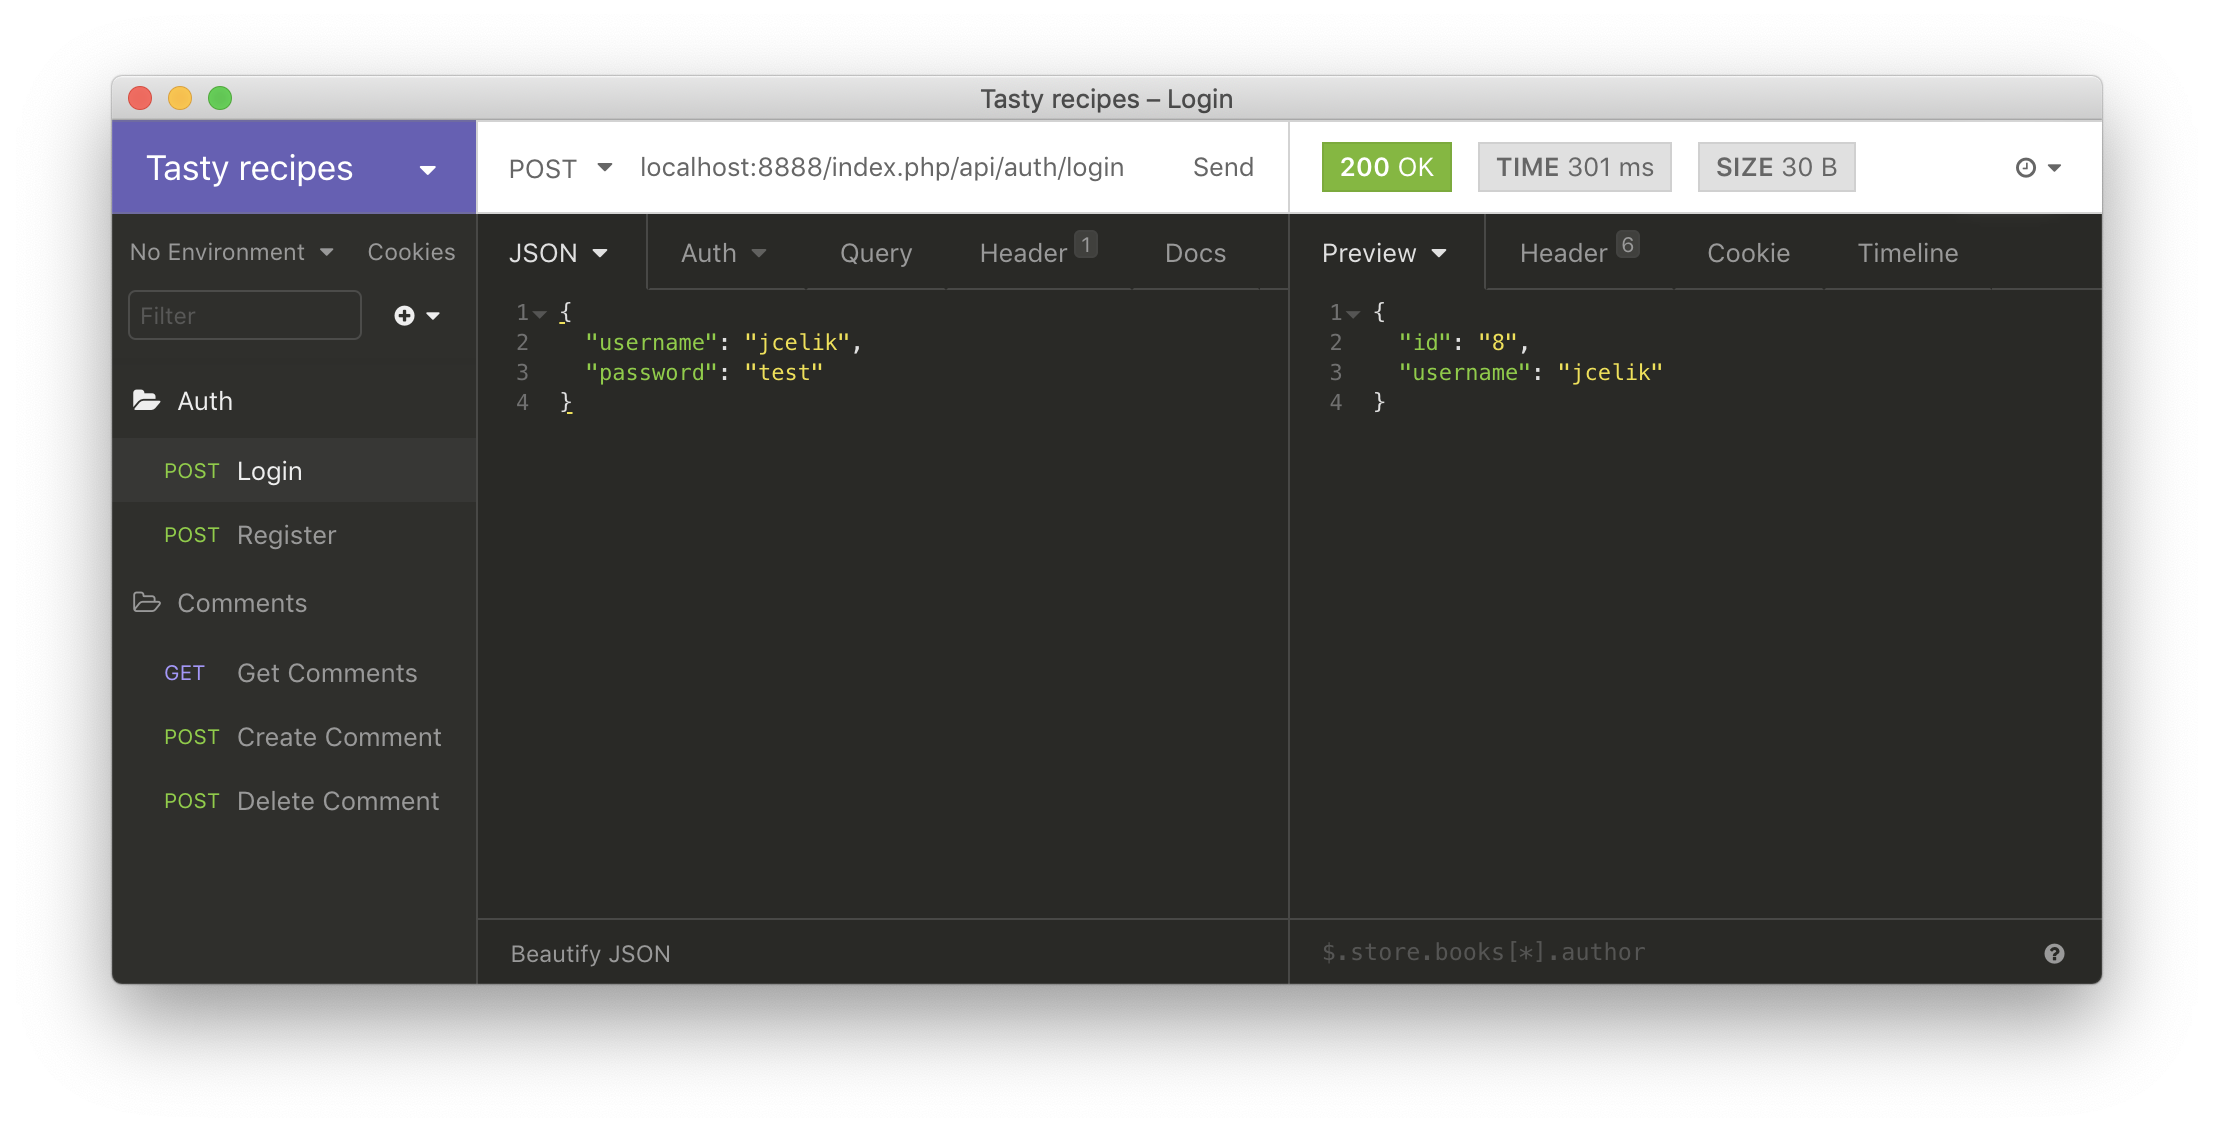
\includegraphics[width=\linewidth]{images/screenshot-insomnia-login.png}
		\caption{Screenshot of Insomnia showing login API call}
		\label{fig:api-login}
	\end{center}
\end{figure}

\newpage
\subsection{Using AJAX for comments}

API routes were added for comments as well. There were three introduced actions:

\begin{itemize}
\item Get all comments related to a recipe.
\item Creating a new comment.
\item Removing a comment.
\end{itemize}

\noindent
No API calls returned HTML. All calls returned data in the JSON format.

\section{Discussion}

There were one mandatory and two optional tasks for this assignment. They were:

\begin{enumerate}
	\item \textbf{Mandatory:} JavaScript Client
	\item \textbf{Optional:} Use a JavaScript Framework
	\item \textbf{Optional:} Long Polling or Server-Sent Events
\end{enumerate}

\noindent
I met the mandatory and the first optional requirement. I truly learned that React is not meant to be used in only a part of a page, even though many claim that it is suitable for that. Elm is another framework that is very suitable for using only for a small piece of an application. It is much more reasonable to create the whole view in only React and only use the server for data. Views can be static files served by a simple CDN. If they get to large they can be split into separate lazy loaded modules and if that is not enough server rendered React or Vue is a good option. To mix creating a view in both PHP and parts of it with JavaScript is unnecessarily complicated.

To create static pages with a good front-end framework is a solution to the performance tasks assigned in the last assignment. If all of the web page consists of static files they can be deployed over a global CDN with a strong cache. The server costs of fetching static resources is very cheap compared to executing PHP or any other language to render an HTML file. In the first assignment I used CloudFlare to cache my web page over 155 data centers. This ensures that my users always get a quick page load, wherever they are. This is a problem I definitely notice with American sites that do not use global CDNs.


\section{Comments About the Course}

I spent most time on this assignment. I understand that there is so much material in this course that it is difficult to capture everything which is the reason that using AJAX to improve the current website was proposed. It is important that JavaScript is introduced in this course. I do however not agree that this was the best assignment, as it required something that is not often done in the industry and is only done as a \textit{hacky} solution. I refer to mixing parts of the view being server rendered and other parts being client rendered.

An alternative assignment could be to improve the recipe page with minor client interactivity. It does not have to be so much. Another assignment could be to create a simple React or Vue page from scratch. Instead of it being complicated it could be something as simple as a todo-app.

I understand that the purpose is to teach the MVVM model, however that is something I do not agree on being very important. Not to say that the MVVM model is not used a lot in the industry but more that it is easy to understand afterwards and the focus could be more on learning JavaScript. JavaScript is an important language to know as the industry is moving towards using it more and more. It is unavoidable compared to PHP.

\end{document}